% !TeX encoding = UTF-8
% !TeX spellcheck = russian-aot
% !TeX program = xelatex
\documentclass[14pt, a4paper, titlepage]{extarticle}

\usepackage[english, main=russian]{babel}
\usepackage{fontspec}
\setmainfont{Times New Roman}
\usepackage[left=30mm, right=15mm, top=20mm, bottom=20mm]{geometry}

\usepackage{microtype}
\usepackage{lettrine}
\renewcommand{\LettrineTextFont}{\upshape}
\usepackage{graphicx}
\usepackage{float}

\usepackage{pgfplots} % Графики
\pgfplotsset{width=.8\textwidth, compat=1.9}

\usepackage{authblk}

\usepackage{csquotes}
\usepackage[left={<<}, right={>>}, leftsub={„}, rightsub={“}]{dirtytalk}
\usepackage[backend=bibtex]{biblatex}
\addbibresource{source.bib}

\linespread{1.3}
\righthyphenmin=2
\parskip=0pt
\parindent=1.25cm

\title{Моделирование систем. Практика 5. Вариант 1}
\author{Р.\,Абдуллин, В.\,Верхотуров \\  БСБО-05-20}
\affil{РТУ МИРЭА}

\usepackage{hyperref}
\hypersetup{pdftitle={Моделирование систем. Практика 5}, pdfauthor={Р. Абдуллин, В. Верхотуров}}

\begin{document}
	\maketitle
	
	\section{Модель}
	
	\begin{figure}[H]
		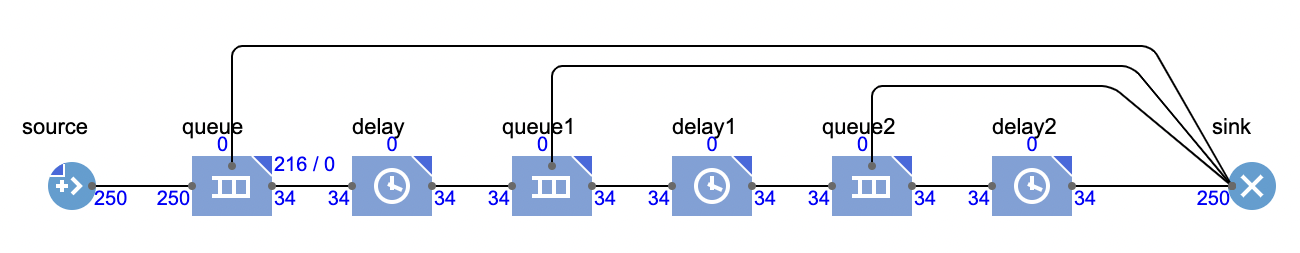
\includegraphics[width=.9\textwidth]{model}
		\caption{Конвейерная вычислительная система}
	\end{figure}

	\begin{figure}[H]
		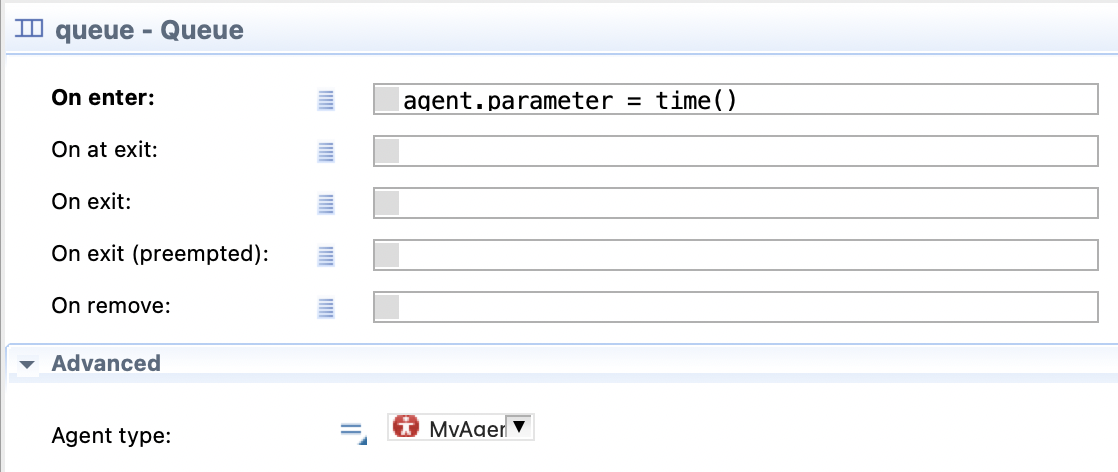
\includegraphics[width=.9\textwidth]{code1}
		\caption{Триггер при входе агента в первую очередь}
	\end{figure}

	\begin{figure}[H]
		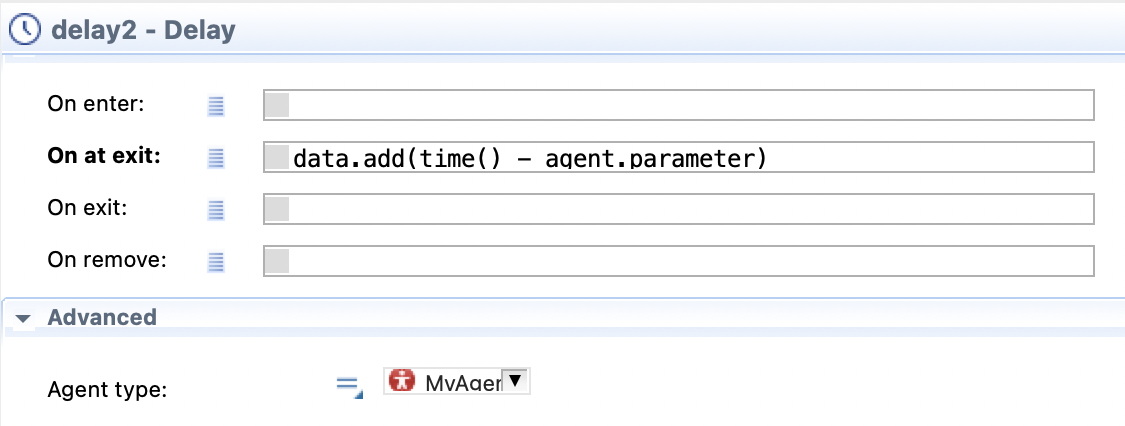
\includegraphics[width=.9\textwidth]{code2}
		\caption{Триггер при выходе агента из последнего процесса}
	\end{figure}
	
	\section{Описание модели}
	
	\begin{description}
		\item[Правило прибытия (сек.)] Интенсивность, 3;
		\item[Максимальное кол-во сообщений] 250;
		\item[] Размеры:
		\begin{description}
			\item[буфера \textnumero~1] 30;
			\item[буфера \textnumero~2] 15;
			\item[буфера \textnumero~3] 50;
		\end{description}
		\item[] Время обработки:
		\begin{description}
			\item[процессора \textnumero~1] 25;
			\item[процессора \textnumero~2] 15;
			\item[процессора \textnumero~3] 5;
			
		\end{description}
		\item[Изучаемый параметр] время нахождения в системе.
	\end{description}
	
	\section{Метод распределения}
	
	\begin{figure}[H]
		\centering
		\begin{tikzpicture}
			\begin{axis}[legend pos = north west, axis lines = left, grid = both, xlabel = $t$, ylabel = {$y$}, ymax=4, ymin=0, xmax=83, xmin=0]
				\addplot [domain=0:100, samples=100, color=red]{3+x*0};
				\addlegendentry{\(3\)};
			\end{axis}
		\end{tikzpicture}
		\caption{Функция, описывающая распределение плотности}
	\end{figure}
	
	\section{Гистограмма, логи временных интервалов, данные гистограммы}
	
	\begin{figure}[H]
		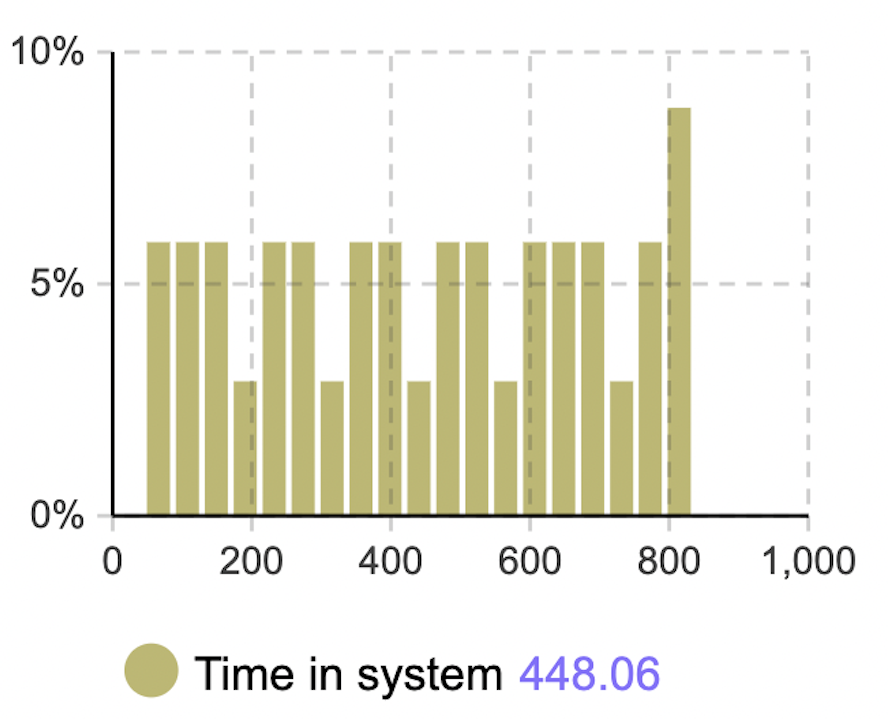
\includegraphics[width=.9\textwidth]{hist}
		\caption{Гистограмма времени нахождения  в системе}
	\end{figure}

	\begin{figure}[H]
		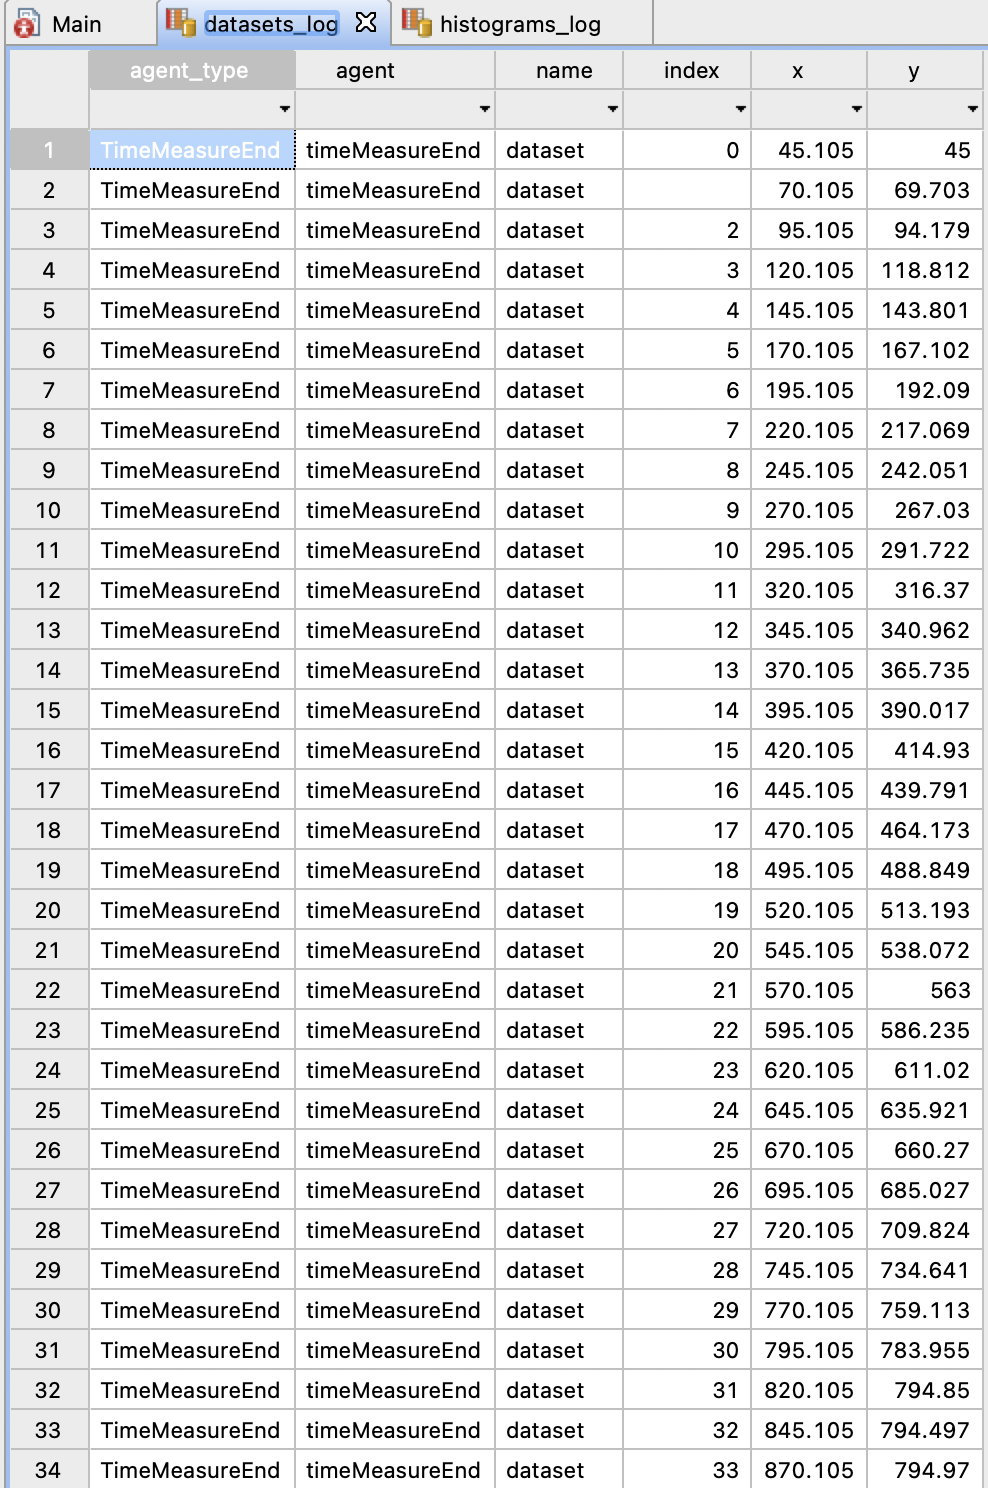
\includegraphics[width=.9\textwidth]{datasets_log}
		\caption{Логи временных интервалов при выходе из системы}
	\end{figure}

	\begin{figure}[H]
		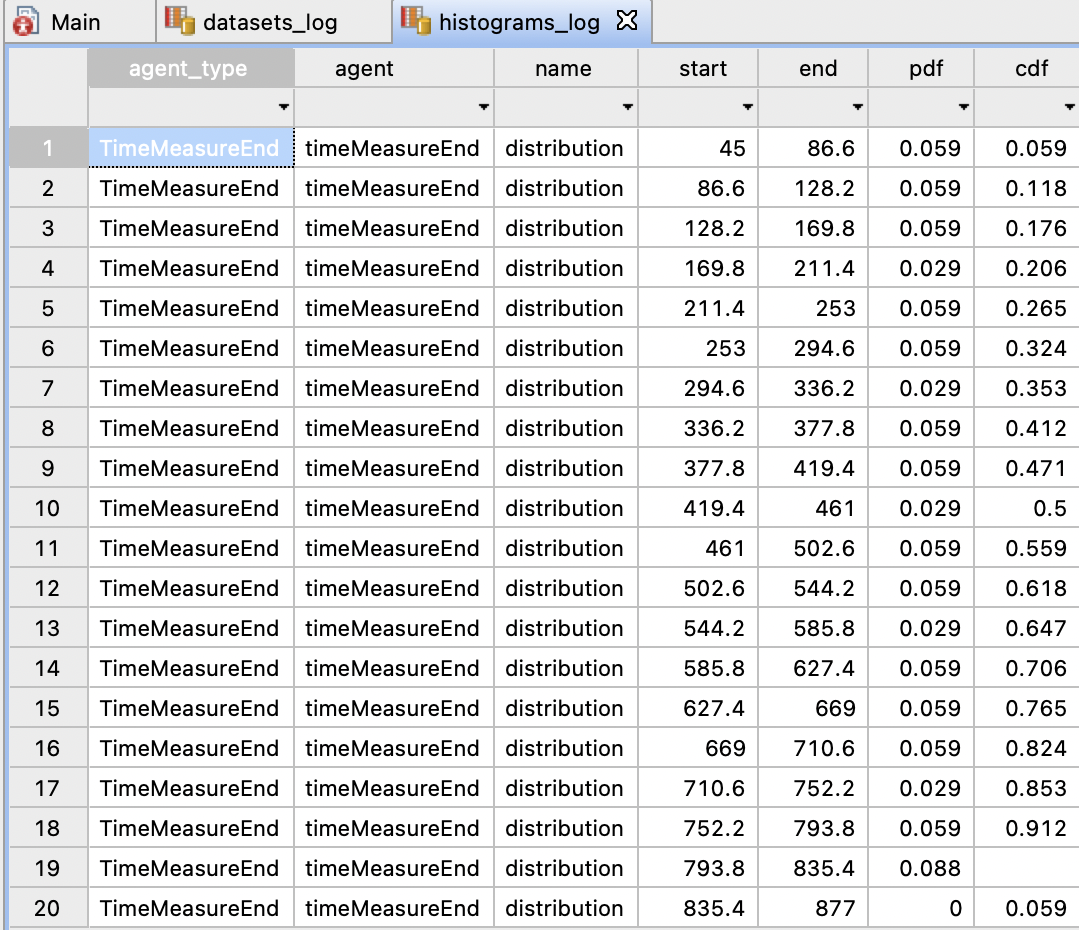
\includegraphics[width=.9\textwidth]{histograms_log}
		\caption{Данные гистограммы}
	\end{figure}
	
	\section{Анализ системы}
	
	216 сообщений были утеряны в буфере 1. Возможно распараллеливание процесса 1 или буфера 1.
	
	\section{Вывод}
	
	Построена и исследована модель конвейерных вычислительных систем, проведён ее анализ.
	
	
	\printbibliography
	
\end{document}